\documentclass[11pt]{article}
\usepackage[a4paper,margin=2cm]{geometry}
\usepackage{graphicx,booktabs,amsmath,float,caption}
\usepackage[hidelinks]{hyperref}
\setlength{\parskip}{4pt}\setlength{\parindent}{0pt}

\title{\textbf{PRML Lab 4 --- Bayes Classification}}
\author{Aryan Tiwari (B20AI056)\\CSL2050 Pattern Recognition \& Machine Learning, Winter 2022}
\date{}

\begin{document}
\maketitle

\section*{Question 1 --- Naive Bayes on the Titanic dataset}

\textbf{1. Pre-processing and column selection.} 891 passengers, 38.4\% survived.
\begin{itemize}\itemsep0pt
\item \emph{Dropped:} \texttt{PassengerId}, \texttt{Name}, \texttt{Ticket} are identifiers with no generalisable signal.
\texttt{Cabin} is 77\% missing, so only a binary \texttt{HasCabin} flag is kept (a recorded cabin mostly means first class).
\item \emph{Missing values:} the 2 missing \texttt{Embarked} values are set to the mode (S). The 177 missing ages are filled with the median age for the
passenger's \emph{title} (Mr/Mrs/Miss/Master/rare), which is much more informative than one global median ---
``Master'' always means a boy. The title itself is not used as a feature: it nearly duplicates \texttt{Sex}, and Naive Bayes would count that evidence twice.
\item \emph{Transform:} \texttt{Fare} is heavily right-skewed, so it is modelled as $\log(1+\text{Fare})$.
\end{itemize}
Final features: \texttt{Pclass}, \texttt{Sex}, \texttt{Embarked}, \texttt{HasCabin} (categorical); \texttt{Age}, \texttt{LogFare} (continuous).
80:20 stratified split (712 / 179).

\begin{figure}[H]\centering
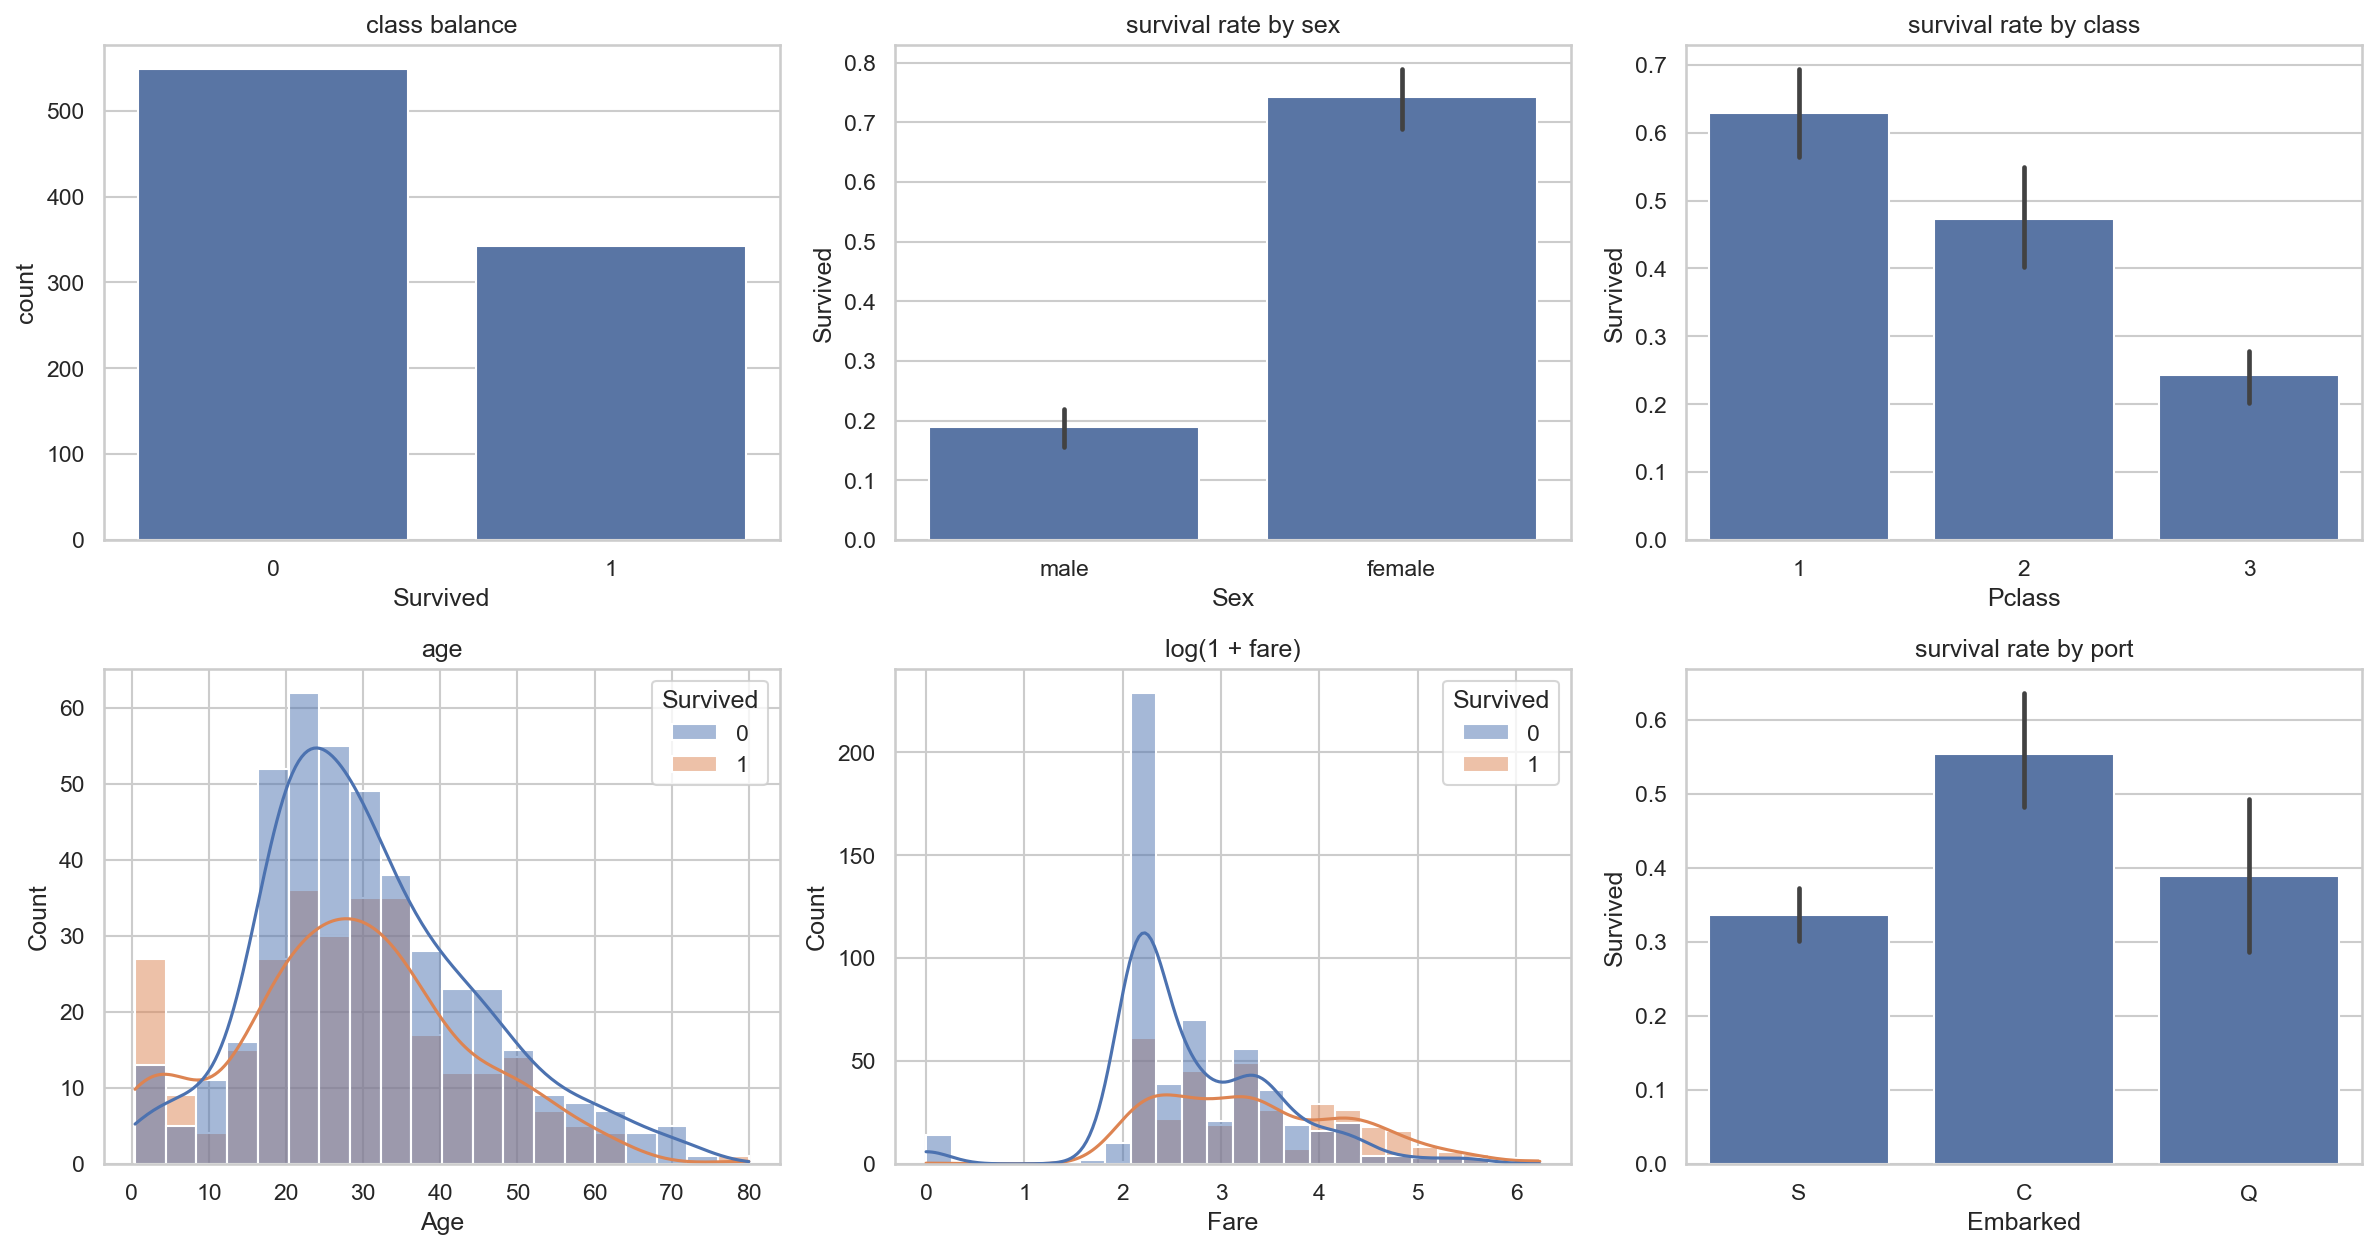
\includegraphics[width=0.95\linewidth]{figures/q1_eda.png}
\caption{Sex and class are the strongest signals (74\% of women survived vs.\ 19\% of men; 63\% of 1st class vs.\ 24\% of 3rd).}
\end{figure}

\textbf{2. Choice of variant: Mixed Naive Bayes.} The features are of mixed type. A Gaussian likelihood on
\texttt{Sex} or \texttt{Embarked} is meaningless, and binning \texttt{Age}/\texttt{Fare} to fit a purely categorical model throws
information away. I therefore use a \textbf{categorical likelihood with Laplace smoothing} for the discrete features and a
\textbf{Gaussian likelihood} for the continuous ones (within each class, age and log-fare are unimodal and close to symmetric).
Under the naive independence assumption the two parts simply add in log space:
\[
\log P(y\mid x) \propto \log P(y) + \sum_{j\in\text{cat}} \log P(x_j\mid y) + \sum_{j\in\text{cont}} \log \mathcal{N}(x_j;\mu_{jy},\sigma^2_{jy}).
\]

\textbf{3. Scratch implementation.} Training stores the log priors, a smoothed probability table per categorical feature and class
(with a fall-back probability for categories never seen in training), and a per-class mean and variance for each continuous feature.
Prediction sums the log terms and normalises with the log-sum-exp trick. The learnt tables match the EDA: for example,
$P(\text{female}\mid\text{survived}) = 0.687$ vs.\ $P(\text{female}\mid\text{died}) = 0.138$.
Test accuracy: \textbf{78.8\%} (train 75.7\%).

\textbf{4--5. 5-fold cross-validation and top-class probabilities.}
\begin{table}[H]\centering
\begin{tabular}{lccccc|c}\toprule
 & Fold 1 & 2 & 3 & 4 & 5 & Mean\\\midrule
Accuracy & 0.741 & 0.741 & 0.761 & 0.739 & 0.796 & \textbf{0.756}\\
Precision & 0.673 & 0.680 & 0.679 & 0.655 & 0.760 & 0.689\\
Recall & 0.636 & 0.618 & 0.704 & 0.667 & 0.691 & 0.663\\
F1 & 0.654 & 0.648 & 0.691 & 0.661 & 0.724 & 0.675\\\bottomrule
\end{tabular}
\end{table}

The folds are consistent (accuracy 0.74--0.80). Recall is lower than precision: the model misses some survivors, typically
men in the upper classes, because the strong \texttt{Sex} likelihood pushes every man towards ``died''. For each of the 179 test rows the
probability of the top class was computed and saved to \texttt{test\_top\_class\_probabilities.csv}. The mean top-class probability
is 0.834. On the 84 rows where it exceeds 0.9 the model is right 88.1\% of the time, so it is somewhat over-confident, which is
expected when correlated features (class, fare, cabin) are treated as independent evidence.

\begin{figure}[H]\centering
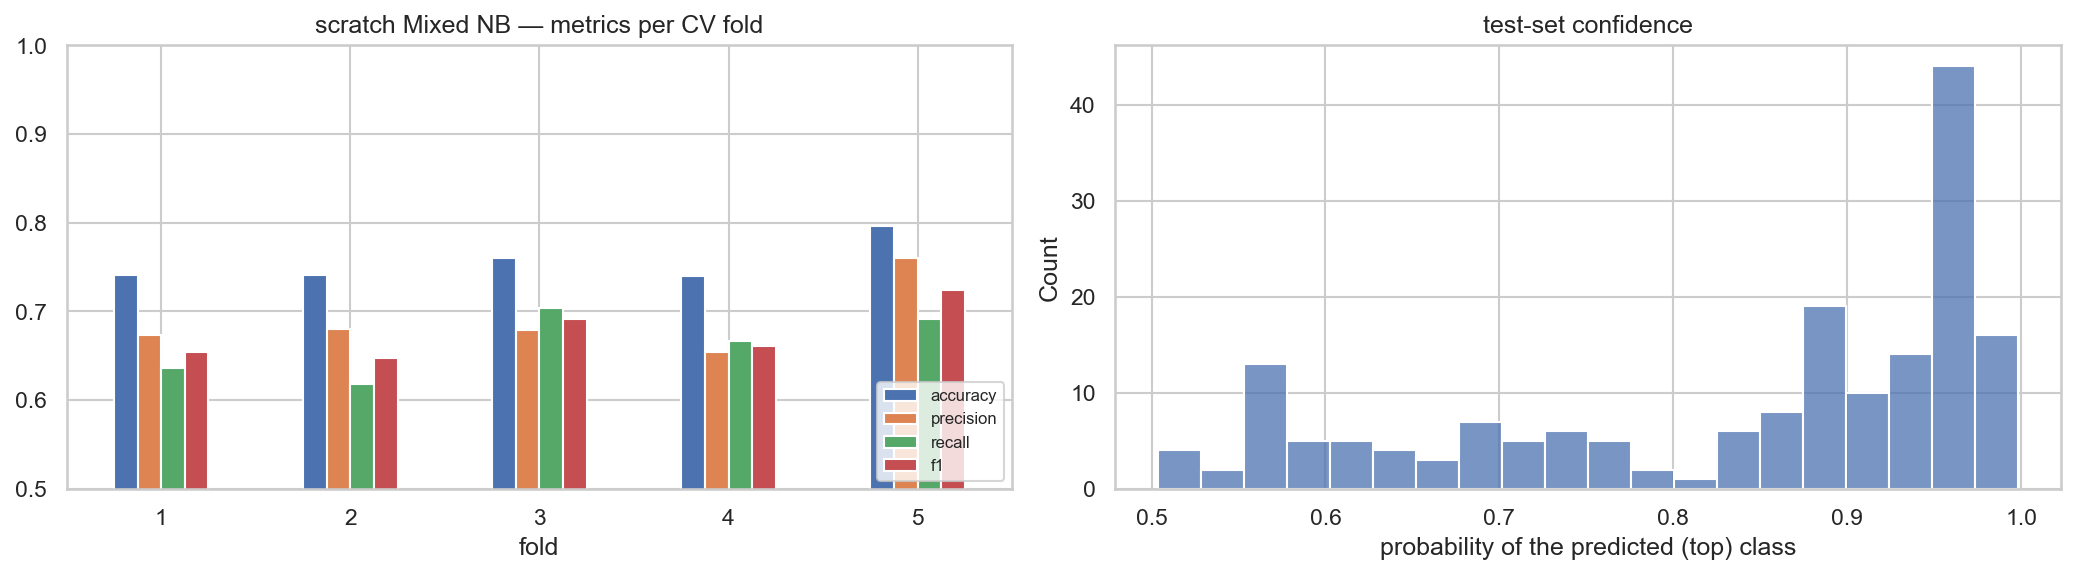
\includegraphics[width=0.95\linewidth]{figures/q1_cv_nb.png}
\caption{Metrics per CV fold (left) and distribution of top-class probabilities on the test set (right).}
\end{figure}

\textbf{6. Scratch vs.\ scikit-learn.} I rebuilt the same model from sklearn parts (\texttt{CategoricalNB} with $\alpha=1$ plus
\texttt{GaussianNB}, adding their log-probabilities and subtracting the duplicated prior once). The predictions agree on
\textbf{100\%} of test rows and the probabilities differ by at most $10^{-10}$, so the scratch implementation is correct. For comparison,
a plain \texttt{GaussianNB} on all features (categoricals as integers) reaches a similar CV accuracy (0.763) but only 0.760 on the test set
compared with 0.788 for the mixed model. It trades precision for recall because it misreads the categorical features as continuous.

\textbf{7. Other models.}
\begin{table}[H]\centering
\begin{tabular}{lccccc}\toprule
Model & CV acc. & CV precision & CV recall & CV F1 & Test acc.\\\midrule
Mixed NB (scratch) & 0.756 & 0.689 & 0.663 & 0.675 & \textbf{0.788}\\
Logistic regression & 0.808 & 0.755 & 0.736 & 0.744 & 0.749\\
Random forest (300 trees, depth 6) & \textbf{0.820} & \textbf{0.806} & 0.700 & \textbf{0.748} & 0.771\\\bottomrule
\end{tabular}
\end{table}

\begin{figure}[H]\centering
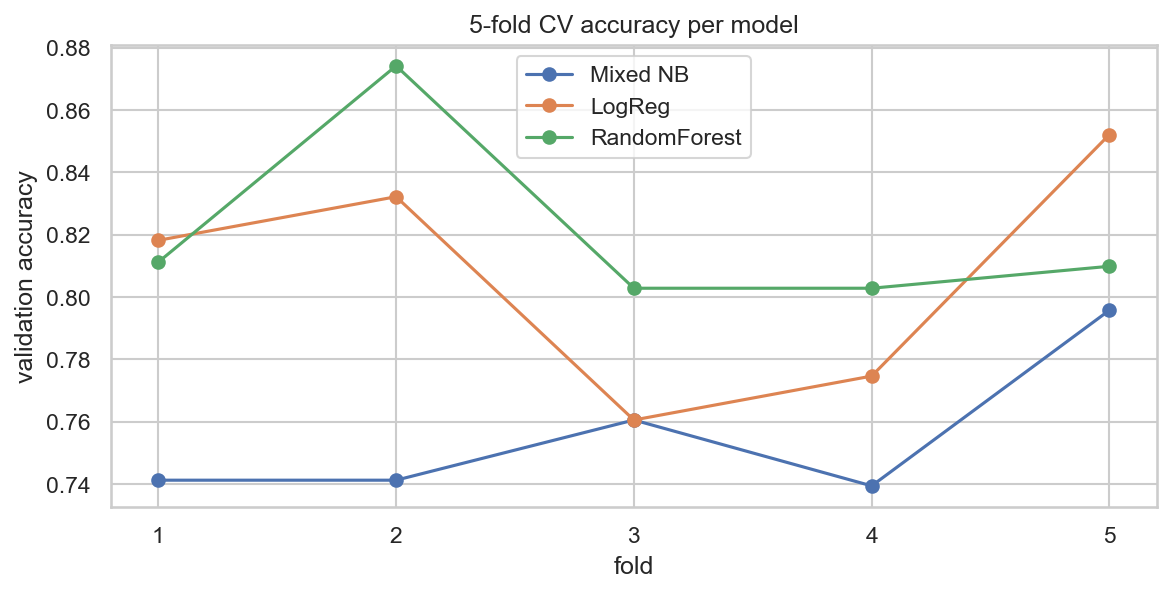
\includegraphics[width=0.6\linewidth]{figures/q1_models.png}
\caption{Validation accuracy per fold for the three models.}
\end{figure}

In cross-validation the discriminative models beat Naive Bayes by about 5--6 points. They do not assume the features are independent, and the forest can
learn interactions such as ``male \emph{and} 1st class'' or ``child \emph{and} 3rd class''. On this particular 179-row test split Naive Bayes
happens to score highest, but each test row is worth 0.56 points, so differences of a few rows are within noise. Cross-validation over five
folds is the more reliable comparison. Naive Bayes is still a strong baseline: it has very few parameters, needs no tuning, and
its probabilities are easy to interpret.

\section*{Question 2 --- Seeds dataset (NumPy / pandas / Matplotlib / Seaborn only)}

210 wheat kernels, 7 geometric features, 3 balanced classes (70 each).

\textbf{a. Distributions.} Area, perimeter, kernel length/width and groove length separate the classes well (class 3 is smallest,
class 2 largest). Compactness and asymmetry overlap much more.

\begin{figure}[H]\centering
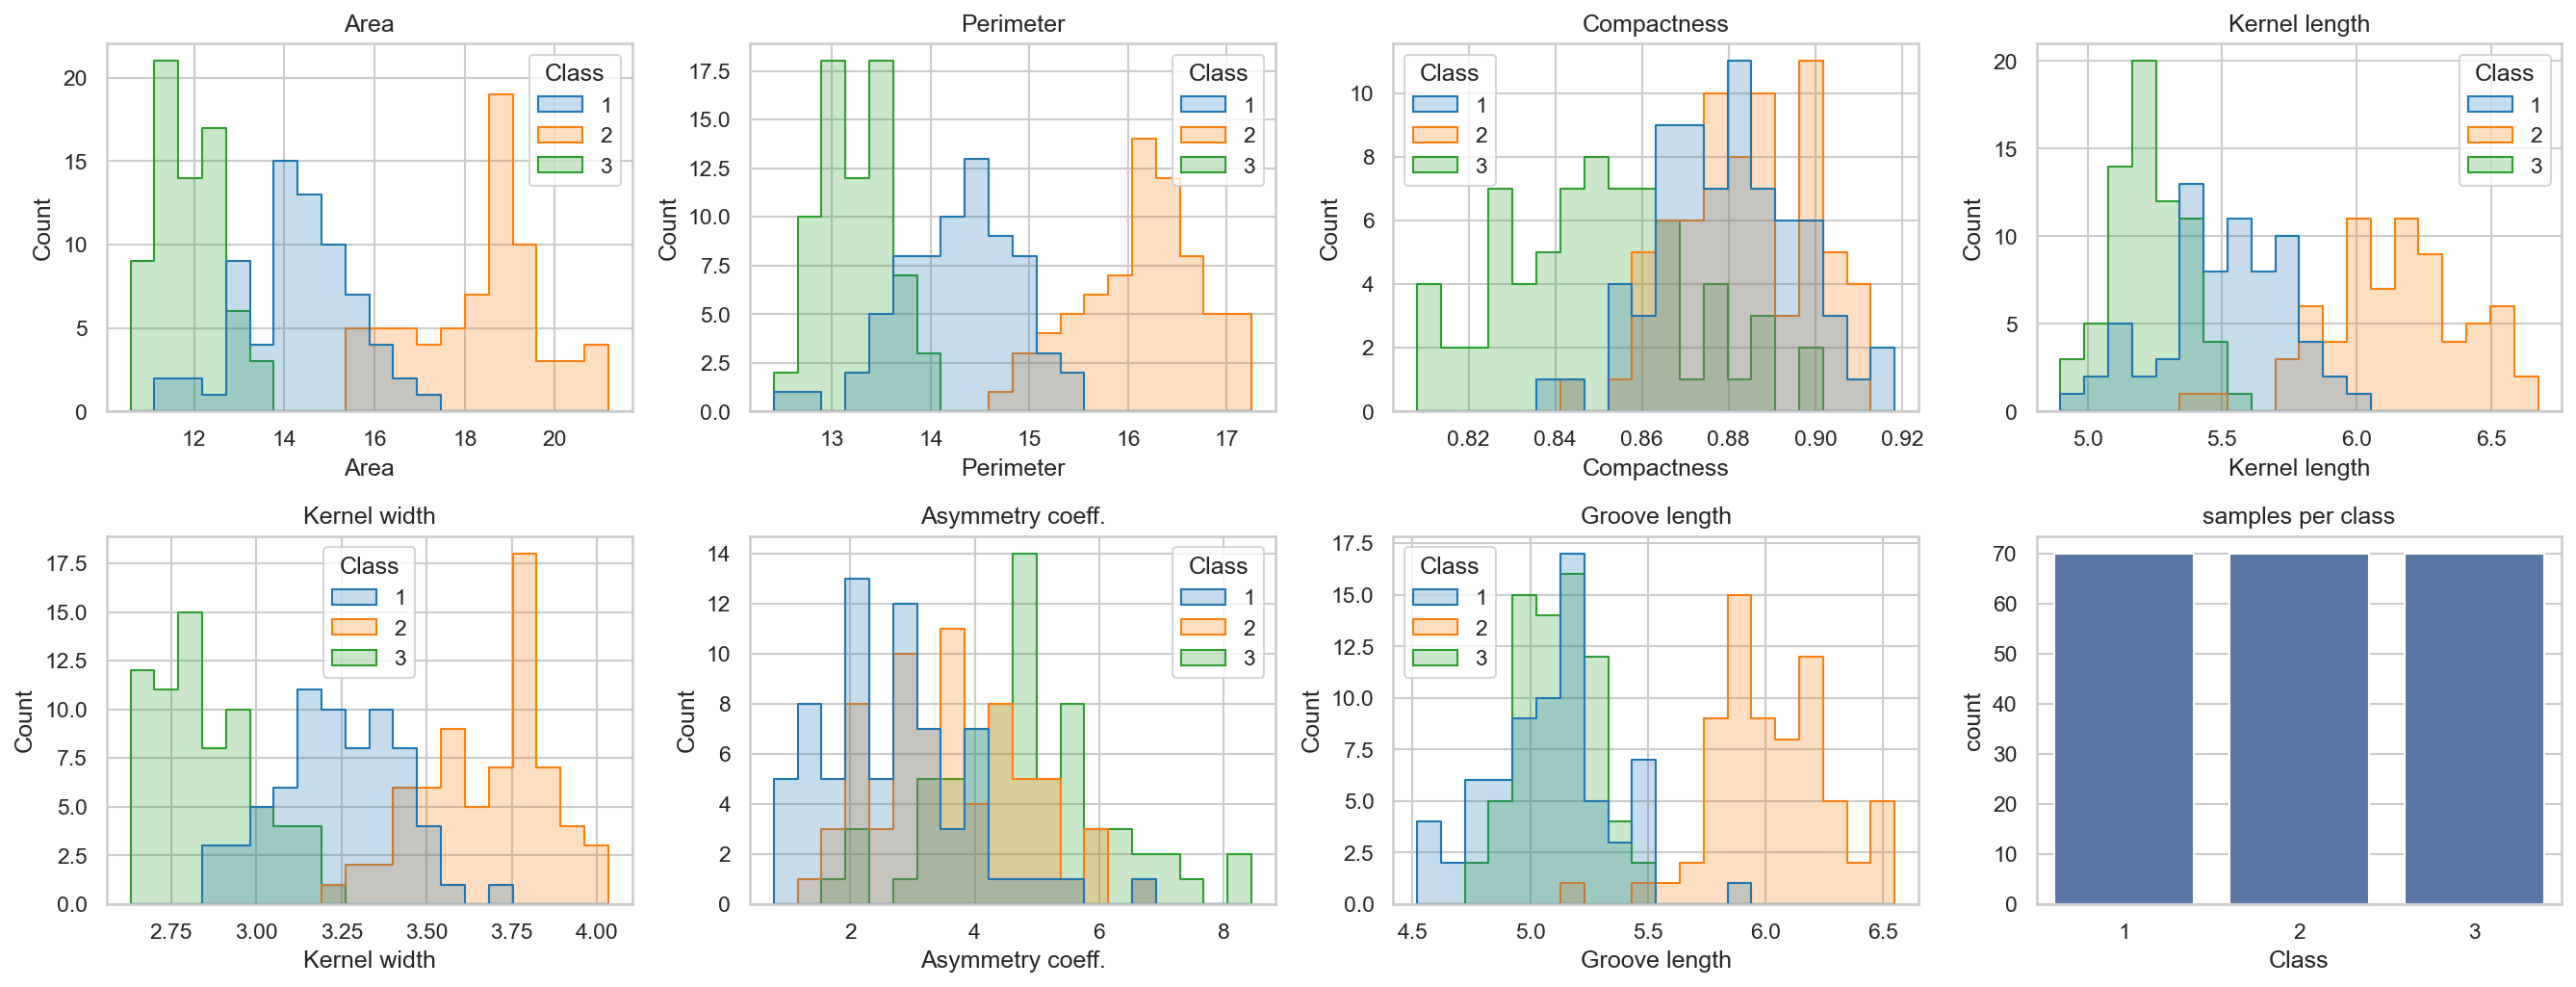
\includegraphics[width=\linewidth]{figures/q2a_distribution.png}
\caption{Per-class histograms of each feature.}
\end{figure}

\textbf{b. Priors.} $P(1)=P(2)=P(3)=1/3$, because the classes are perfectly balanced.

\textbf{c. Discretisation from scratch.} Each feature is cut into equal-width bins between its minimum and maximum, using only plain
Python and NumPy arithmetic. The number of bins follows \textbf{Sturges' rule}, $k=\lceil\log_2 n\rceil+1 = 9$ for $n=210$. This
keeps each class's shape while leaving about 23 samples per bin on average, which matters because each bin probability is estimated
separately for every class. Values equal to the maximum go into the last bin.

\textbf{d. Likelihoods.} $P(\text{bin}=b\mid c)$ for every feature, bin and class, with Laplace (+1) smoothing so that an empty bin
cannot set the whole product to zero. For example, for Area:

\begin{table}[H]\centering\small
\begin{tabular}{lccccccccc}\toprule
 & bin 0 & 1 & 2 & 3 & 4 & 5 & 6 & 7 & 8\\\midrule
class 1 & 0.038 & 0.114 & 0.266 & \textbf{0.342} & 0.165 & 0.038 & 0.013 & 0.013 & 0.013\\
class 2 & 0.013 & 0.013 & 0.013 & 0.013 & 0.139 & 0.165 & 0.228 & \textbf{0.291} & 0.127\\
class 3 & 0.418 & \textbf{0.430} & 0.076 & 0.013 & 0.013 & 0.013 & 0.013 & 0.013 & 0.013\\\bottomrule
\end{tabular}
\end{table}

\textbf{e. Counts per bin vs.\ the distribution.} The binned counts keep the shape of the histograms in (a): class 3 sits in the lowest
area/perimeter bins, class 2 in the highest, class 1 in between. Binning coarsens the detail but keeps the information about which class sits where.
Compactness and asymmetry overlap across classes in both plots, so they contribute the least evidence.

\begin{figure}[H]\centering
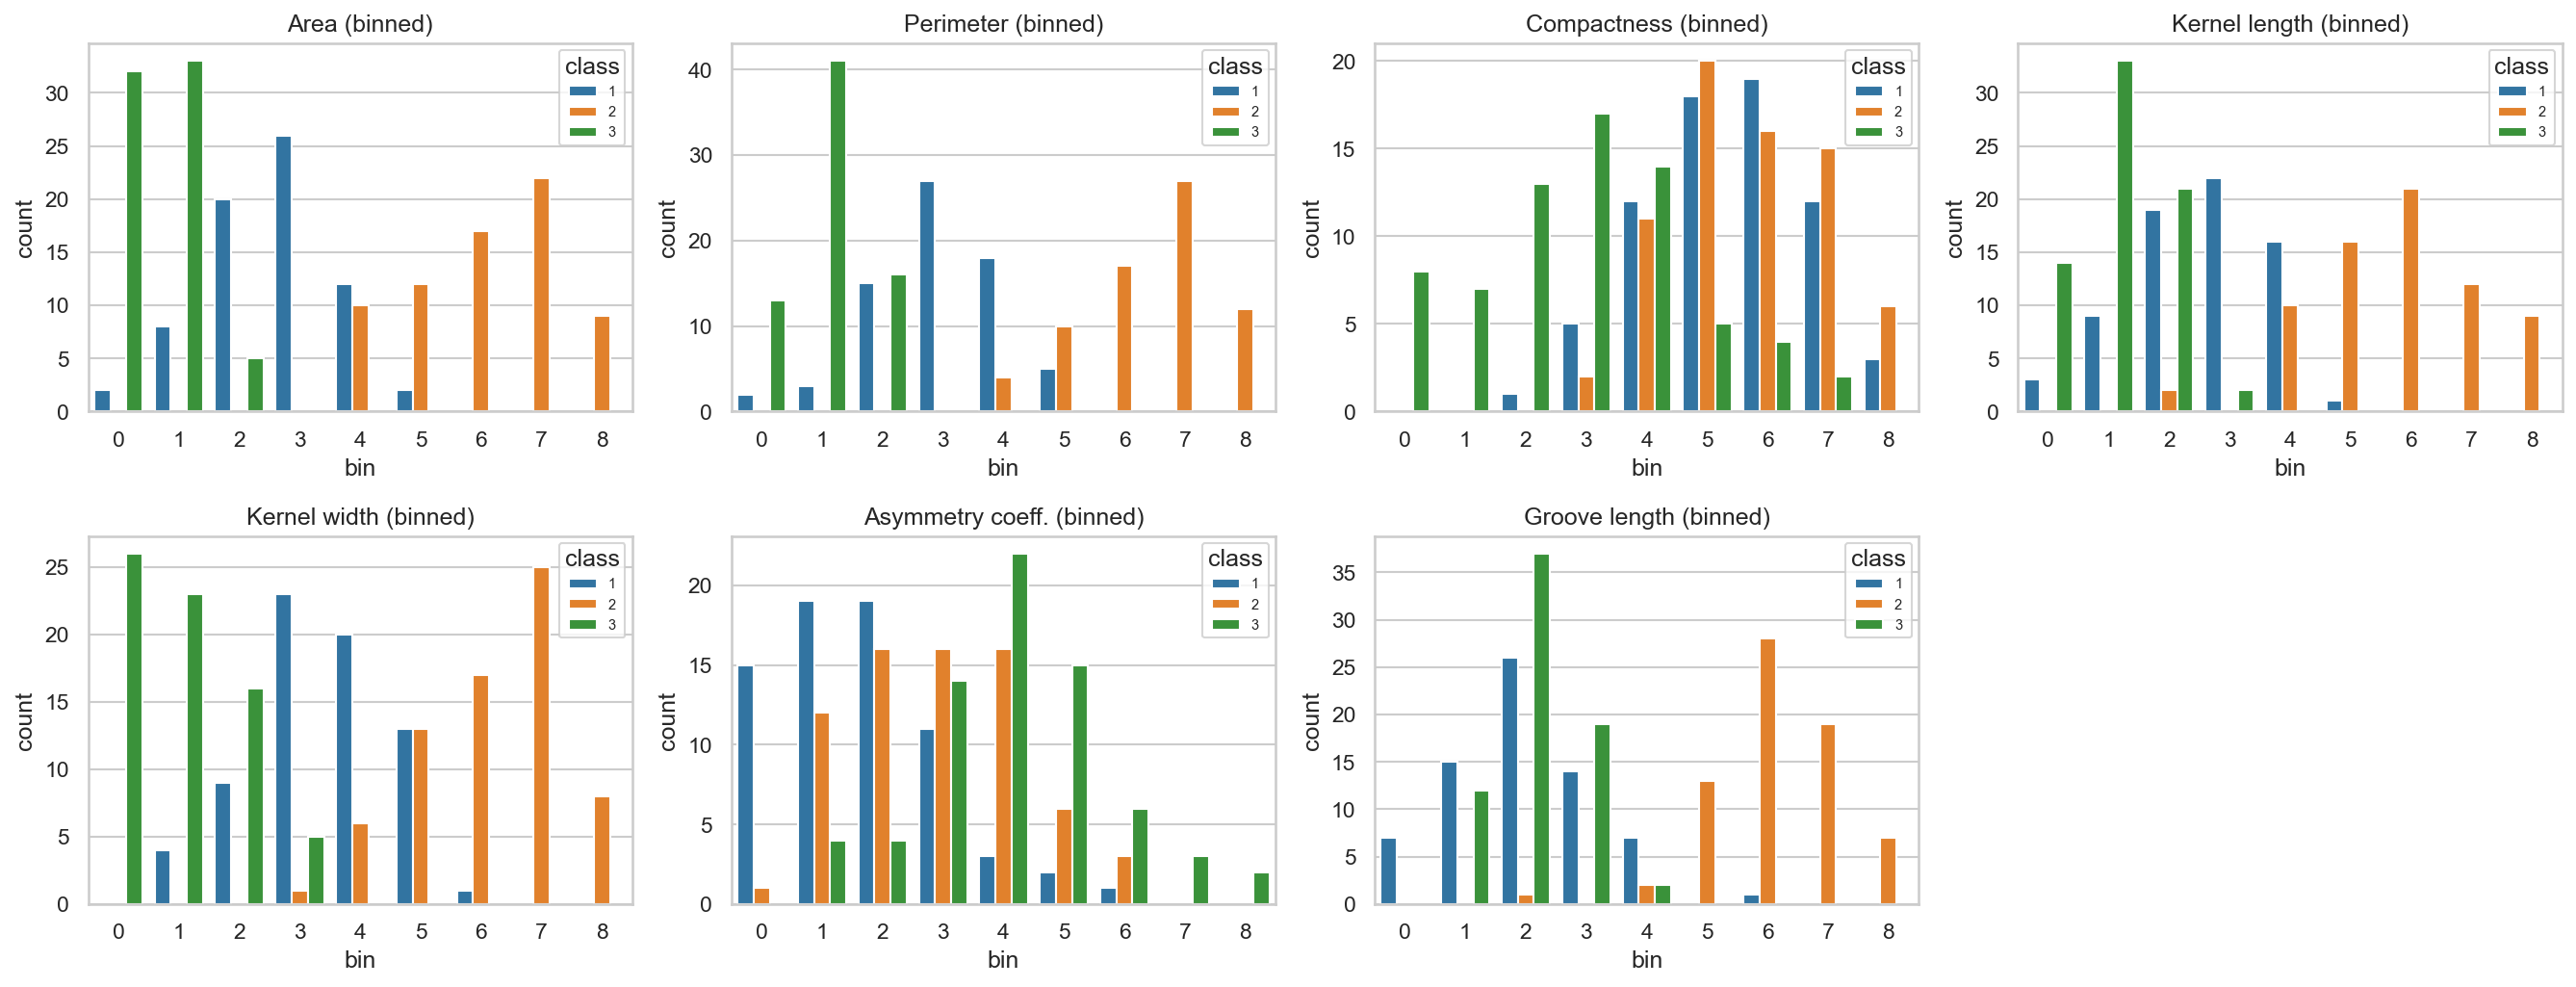
\includegraphics[width=\linewidth]{figures/q2e_counts.png}
\caption{Count of each bin value per class.}
\end{figure}

\textbf{f. Posterior probabilities.} $P(c\mid x)\propto P(c)\prod_j P(x_j\mid c)$, computed in log space and normalised. Bin edges,
priors and likelihoods are estimated on a random 70\% (147 samples) and the posteriors are evaluated on the held-out 30\% (63 samples).
Held-out accuracy is \textbf{95.2\%} (train 91.2\%).

\begin{figure}[H]\centering
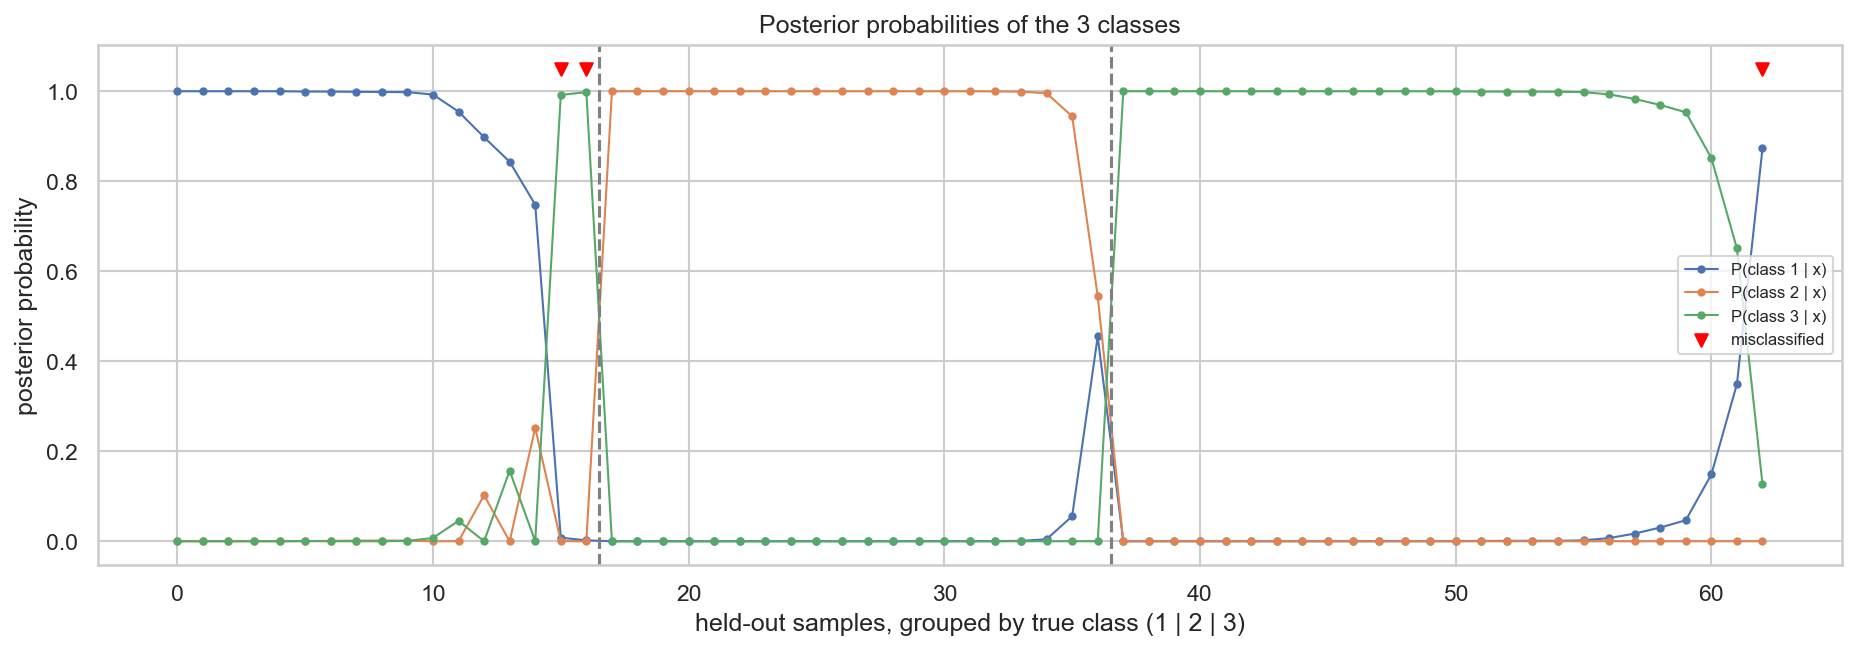
\includegraphics[width=\linewidth]{figures/q2f_posteriors.png}
\caption{Posteriors of all three classes for each held-out kernel, grouped by true class and sorted by confidence in the true class.}
\end{figure}

\textbf{Analysis.} Most kernels get a posterior close to 1 for their true class, because seven features each contribute a strong
likelihood ratio and the naive product multiplies them together. All 20 class-2 kernels are classified correctly: class 2 is the
largest variety and does not overlap with the others in the size features. The three errors are between classes 1 and 3 (two
class-1 kernels predicted as class 3, one the other way round), which overlap in the small-to-medium size bins. Two of these errors
are made with posterior $>0.99$. This is the familiar over-confidence of Naive Bayes: area, perimeter, length and width are strongly
correlated, so the model counts what is essentially one ``size'' signal four times.

\end{document}
